\documentclass[a4paper]{article}

%%%%%%%% CREATE DOCUMENT STRUCTURE %%%%%%%%
%% Language and font encodings
\usepackage[english]{babel}
\usepackage[utf8x]{inputenc}
\usepackage[T1]{fontenc}
%\usepackage{subfig}

%% Sets page size and margins
\usepackage[a4paper,top=3cm,bottom=2cm,left=2cm,right=2cm,marginparwidth=1.75cm]{geometry}

%% Useful packages
\usepackage{amsmath,amssymb}
\usepackage{graphicx}
\usepackage[colorinlistoftodos]{todonotes}
\usepackage[colorlinks=true, allcolors=blue]{hyperref}
\usepackage{caption}
\usepackage{subcaption}
\usepackage{sectsty}
\usepackage{apacite}
\usepackage{float}
\usepackage{titling} 
\usepackage{blindtext}
\usepackage[square,sort,comma,numbers]{natbib}
\usepackage[colorinlistoftodos]{todonotes}
\usepackage{xcolor}
\definecolor{darkgreen}{rgb}{0.0, 0.4, 0.0}
\usepackage{graphicx}
\newcommand{\norm}[1]{\left\lVert#1\right\rVert}
\DeclareMathOperator{\R}{\mathbb{R}}
\DeclareMathOperator{\E}{\mathbb{E}}
\usepackage{multirow}
\usepackage{listings}
\usepackage{xcolor}

\usepackage{multirow}
\usepackage{colortbl}
\usepackage{hhline}

\definecolor{codegreen}{rgb}{0,0.6,0}
\definecolor{codegray}{rgb}{0.5,0.5,0.5}
\definecolor{codepurple}{rgb}{0.58,0,0.82}
\definecolor{backcolour}{rgb}{0.95,0.95,0.92}

\lstdefinestyle{mystyle}{
	backgroundcolor=\color{backcolour},   
	commentstyle=\color{codegreen},
	keywordstyle=\color{magenta},
	numberstyle=\tiny\color{codegray},
	stringstyle=\color{codepurple},
	basicstyle=\ttfamily\footnotesize,
	breakatwhitespace=false,         
	breaklines=true,                 
	captionpos=b,                    
	keepspaces=true,                 
	numbers=left,                    
	numbersep=5pt,                  
	showspaces=false,                
	showstringspaces=false,
	showtabs=false,                  
	tabsize=2
}

\lstset{style=mystyle}
 



%%%%%%%% DOCUMENT %%%%%%%%
\begin{document}

%%%% Title Page
\begin{titlepage}

\newcommand{\HRule}{\rule{\linewidth}{0.5mm}} 							% horizontal line and its thickness
\center 
 
 
% University


\includegraphics[width=0.15\textwidth]{images/kth_logo.png}\\[0.5cm] 	% University logo

\textsc{\LARGE KTH Royal Institute of Technology}\\[1cm]

% Document info
\textsc{\Large Deep Learning in Datascience}\\[0.2cm]
\textsc{\large DD2424}\\[1cm] 										% Course Code
\HRule \\[0.8cm]
{ \huge \bfseries Assignment 2 (Bonus)}\\[0.7cm]								% Assignment
\HRule \\[2cm]
\large
\emph{Authors:}\\
Ali Banaei Mobarak Abadi\\[1.5cm]													% Author info
{\large \today}\\[5cm]

\vfill 
\end{titlepage}

\section{Introduction}

For the bonus part of this assignment, we focus on enhancing the performance of the model. For this purpose, different techniques such as data augmentation, regularization and increasing the number of hidden nodes were used.

\section{More hidden nodes}

One way to enhance the performance of a network is to add more hidden nodes so the complexity of the model would increase. In order to investigate the effect of the number of hidden nodes, a grid search on the number of hidden nodes and the value for lambda was performed. Since, as mentioned in the instructions, by increasing the complexity of the model, we will increase the probability of overfitting, we may use stronger regularization. So, we have to fine-tune the number of hidden nodes and the regularization parameter jointly. We used the values [10, 50, 70, 100, 150] for dimensionality of the hidden space and [0.0001, 0.001, 0.01, 0.1] for lambda value. For each pair of parameters, a model was trained for eight iterations on all the available training sets and then tested on a disjoint validation set. The results of this search can be found in \autoref{tab:hidden}.



\begin{table}[h]
	\centering
	\caption{Accuracy of the model in grid search on number of hidden nodes and lambda.}
	\label{tab:hidden}
	\begin{tabular}{|c|c|c|c|c|c|} 
		\hline
		\multicolumn{2}{|c|}{\multirow{2}{*}{}} & \multicolumn{4}{c|}{Lambda}   \\ 
		\cline{3-6}
		\multicolumn{2}{|c|}{}                  & 0.0001 & 0.001 & 0.01 & 0.1   \\ 
		\hline
		\multirow{5}{*}{Hidden nodes} & 10      & 0.30   & 0.33  & 0.40 & 0.35  \\ 
		\cline{2-6}
		& 50      & 0.43   & 0.45  & 0.47 & 0.36  \\ 
		\cline{2-6}
		& 70      & 0.45   & 0.46  & 0.48 & 0.36  \\ 
		\cline{2-6}
		& 100     & 0.46   & 0.48  & 0.48 & 0.35  \\ 
		\cline{2-6}
		& 150     & 0.48   & 0.48  & 0.47 & 0.36  \\
		\hline
	\end{tabular}
\end{table}

As we see, increasing the number of hidden nodes seems to benefit us until around 100 nodes. Note that we did not encounter overfitting here since we are training the model only for eight epochs. Also, we must be aware that increasing the training time may help us get a more accurate conclusion, especially considering the fact that more complex models may need more time to train. But based on our available time and computational power, this grid search can be sufficient.

\section{Using Dropout}

Now, we use dropout to regularize the network more. To see the effect of dropout, we trained the same network as exercise 4. The accuracy, cost, and loss during training can be found in \autoref{fig:dropout}. As we can see, the training and validation curves are closer to each other, and we get around 4 percent better accuracy on validation data. However, this value is small, and it is expected that dropout will help us more when we have a wider network with more units.

\begin{figure}[h]
	\centering
	\begin{subfigure}{0.3\textwidth}
		\centering
		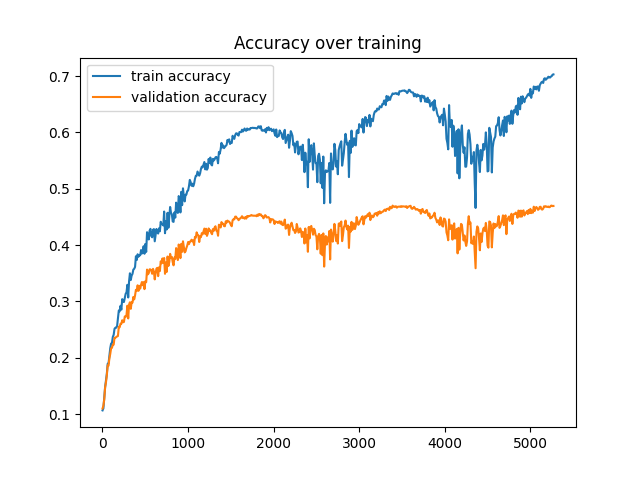
\includegraphics[width=\linewidth]{images/model_of_ex4_dropout__acc.png}
		\caption{}
	\end{subfigure}
	\begin{subfigure}{0.3\textwidth}
		\centering
		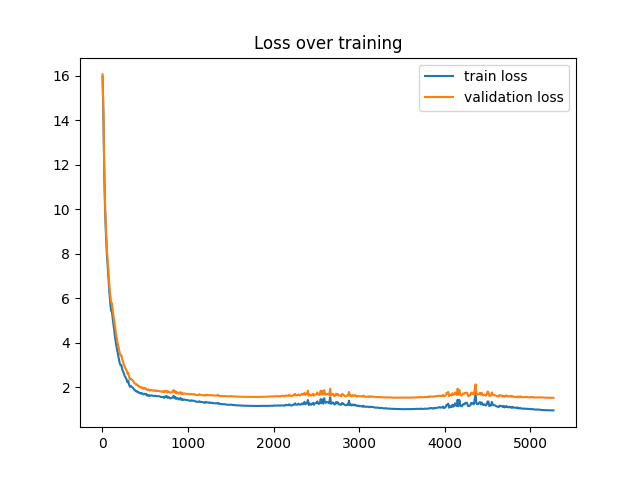
\includegraphics[width=\linewidth]{images/model_of_ex4_dropout__loss.png}
		\caption{}
	\end{subfigure}
	\begin{subfigure}{0.3\textwidth}
		\centering
		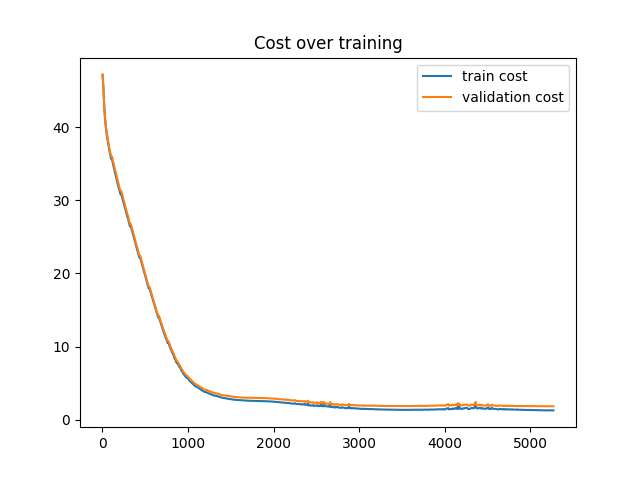
\includegraphics[width=\linewidth]{images/model_of_ex4_dropout__cost.png}
		\caption{}
	\end{subfigure}
	\caption{Exercise 4 with Dropout}
	\label{fig:dropout}
\end{figure}

\section{Data Augmentation}

As another enhancement method, the same way for augmenting the data as the first assignment was used. To check the effect of this method, the same model as exercise 4 was trained. As we can see in \autoref{fig:aug}, the gap was further reduced, and we reached a better performance on the validation set.

\begin{figure}[h]
	\centering
	\begin{subfigure}{0.3\textwidth}
		\centering
		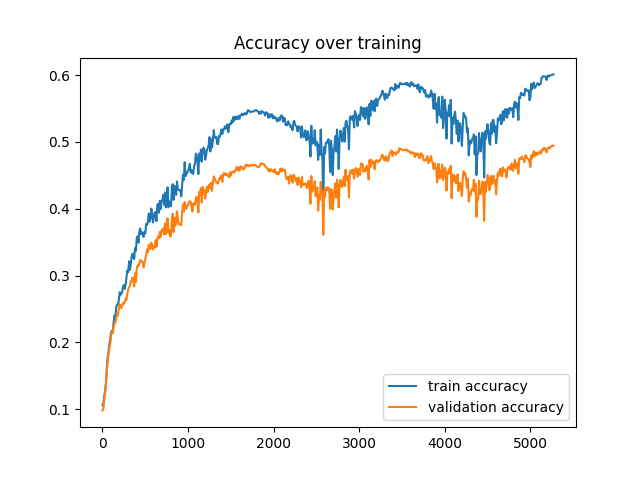
\includegraphics[width=\linewidth]{images/model_of_ex4_fliping__acc.png}
		\caption{}
	\end{subfigure}
	\begin{subfigure}{0.3\textwidth}
		\centering
		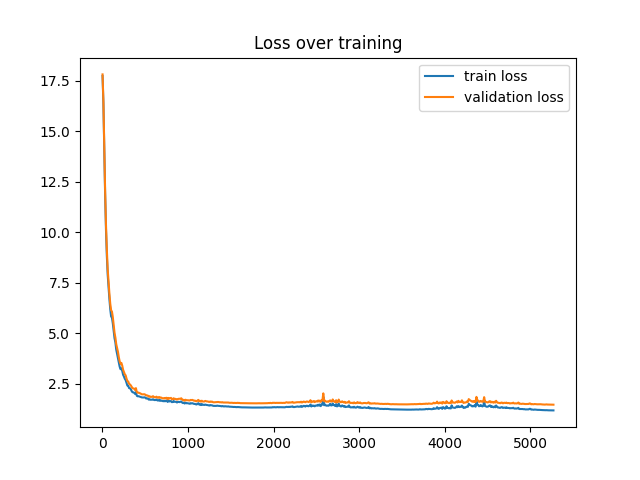
\includegraphics[width=\linewidth]{images/model_of_ex4_fliping__loss.png}
		\caption{}
	\end{subfigure}
	\begin{subfigure}{0.3\textwidth}
		\centering
		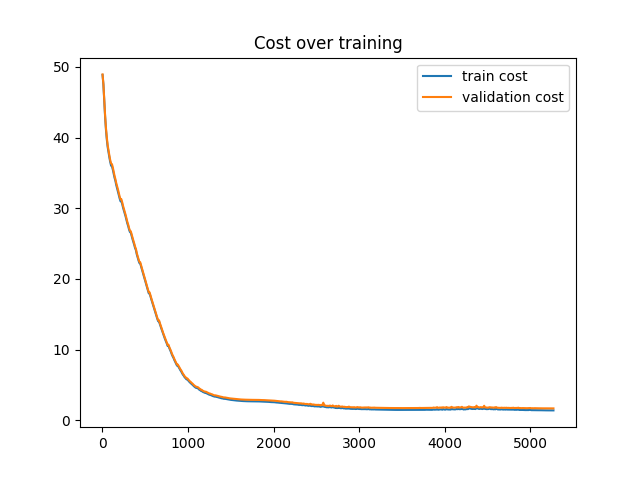
\includegraphics[width=\linewidth]{images/model_of_ex4_fliping__cost.png}
		\caption{}
	\end{subfigure}
	\caption{Exercise 4 with Dropout}
	\label{fig:aug}
\end{figure}

\section{Learning rate decay}
As we proceed with training, it may be a good idea to decrease the max learning rate in our scheduler. For this purpose, the scheduler, after each up and down, multiplies the max learning rate to a factor below 1. \autoref{fig:decay} depicts the learning rate after applying this change.

\begin{figure}[H]
\centering
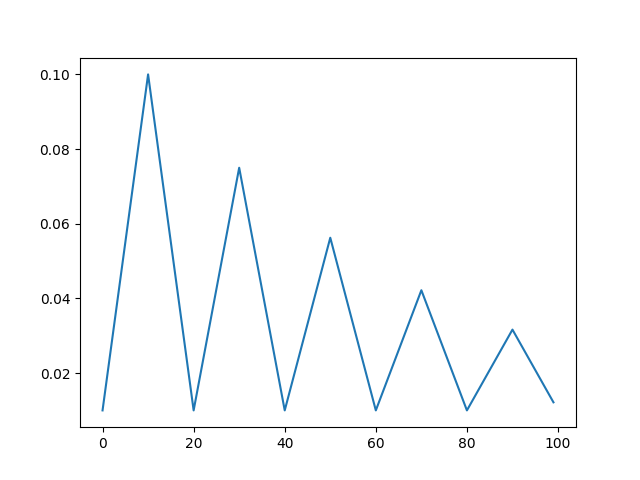
\includegraphics[width=0.5\linewidth]{images/scheduler_decay.png}
\caption{Max learning rate decay}
\label{fig:decay}
\end{figure}

\section{Training a big model}

For the next part, a model with 100 hidden units was trained. In order to prevent overfitting, both data augmentation and dropout were used. For dropout, we turn off the nodes with a probability of 0.3. Also, during training, we decay the max learning rate with a factor of 0.8 after each $2 n_s$. As we can see in \autoref{fig:big}, this model can reach an accuracy of 0.54 after 30 iterations over all the data.


\begin{figure}[h]
	\centering
	\begin{subfigure}{0.3\textwidth}
		\centering
		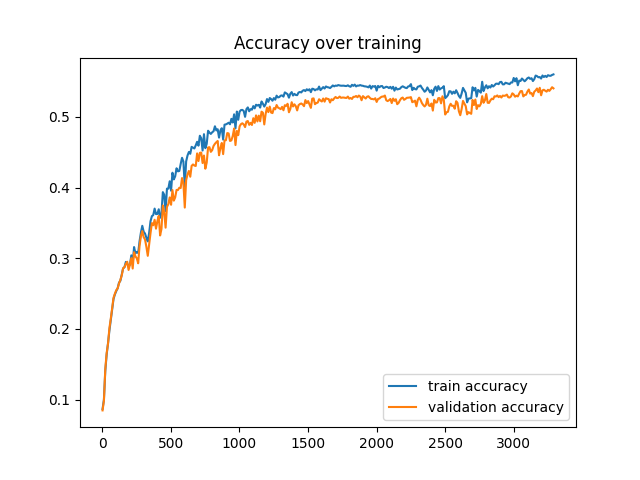
\includegraphics[width=\linewidth]{images/100_node_model_acc.png}
		\caption{}
	\end{subfigure}
	\begin{subfigure}{0.3\textwidth}
		\centering
		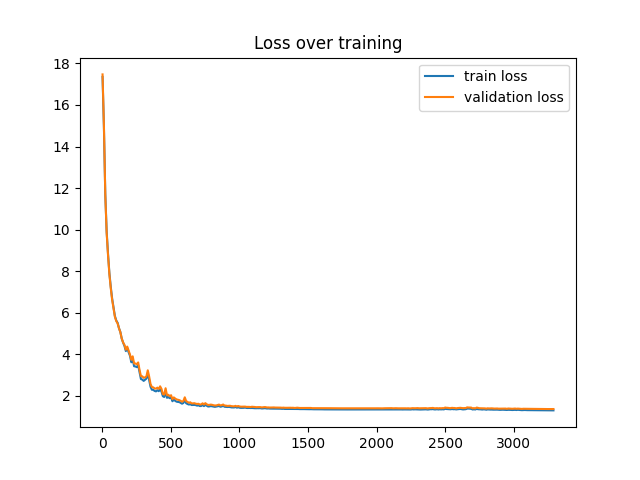
\includegraphics[width=\linewidth]{images/100_node_model_loss.png}
		\caption{}
	\end{subfigure}
	\begin{subfigure}{0.3\textwidth}
		\centering
		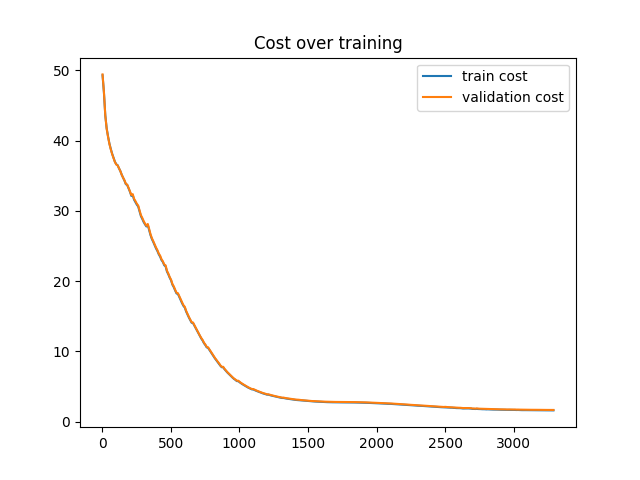
\includegraphics[width=\linewidth]{images/100_node_model_cost.png}
		\caption{}
	\end{subfigure}
	\caption{Exercise 4 with Dropout}
	\label{fig:big}
\end{figure}

\section{Intensive search on hyperparameter tuning}

As the last part of the bonus part, we try to find a good combination of different hyperparameters which performs adequately. One should note that the best way to search for good parameters is to perform a grid search since different parameters can have an effect on each other and cannot be fine-tuned independently. However, here since performing a grid search would exponentially increase the number of models to train, some parameters that are predicted to have a minimal effect on each other are searched independently. We use a model with 120 units in the hidden layer in our search.
In the first step, we find a good value for the factor which we use to decay the max learning rate. For this purpose, values of [0.5, 0.65, 0.8, 0.9] were tested (each model was trained for 20 epochs).  All these values resulted in very close results on our training (longer training may reveal more difference), but the value of 0.8 had the highest accuracy of 0.52.

In the next step, we must find a good combination of values for the dropout parameter and lambda. Since weight decay and dropout are both forms of regularization, it is better to fine-tune them jointly. So, we did a grid search. For each combination of parameters, we trained the model for 20 epochs with a decay of 0.8 for the max learning rate, as we found in the last part. The accuracy of each model can be found in \autoref{tab:final}.




\begin{table}[h]
	\centering
	\caption{Accuracy of the model in grid search Dropout and lambda parameter.}
	\label{tab:final}
	\begin{tabular}{|c|c|c|c|c|} 
		\cline{3-5}
		\multicolumn{2}{c|}{\multirow{2}{*}{}} & \multicolumn{3}{c|}{Lambda}  \\ 
		\cline{3-5}
		\multicolumn{2}{c|}{}                  & 0    & 0.001 & 0.01          \\ 
		\hline
		\multirow{5}{*}{Dropout p} & 1         & 0.47 & 0.49  & 0.51          \\ 
		\cline{2-5}
		& 0.85      & 0.48 & 0.49  & 0.51          \\ 
		\cline{2-5}
		& 0.7       & 0.49 & 0.50  & 0.52          \\ 
		\cline{2-5}
		& 0.55      & 0.48 & 0.49  & 0.52          \\ 
		\cline{2-5}
		& 0.4       & 0.47 & 0.48  & 0.51          \\
		\hline
	\end{tabular}
\end{table}

So, it seems like 0.7 as a dropout parameter and 0.01 as lambda can be a good combination. Finally, we want to see how many iterations we must train our network. Therefore, a model with the parameters we found is trained for a long time. We then look at the graphs and see when the model reaches a flat area or if there is overfitting. The model was trained for 80 epochs and [] depicts the records during training. As we see, there is no sign of overfitting to the training data. However, after 40 epochs, it looks like we do not experience much increase in the model's performance. This model reached the performance of 0.55 on test data.


\begin{figure}[h]
	\centering
	\begin{subfigure}{0.3\textwidth}
		\centering
		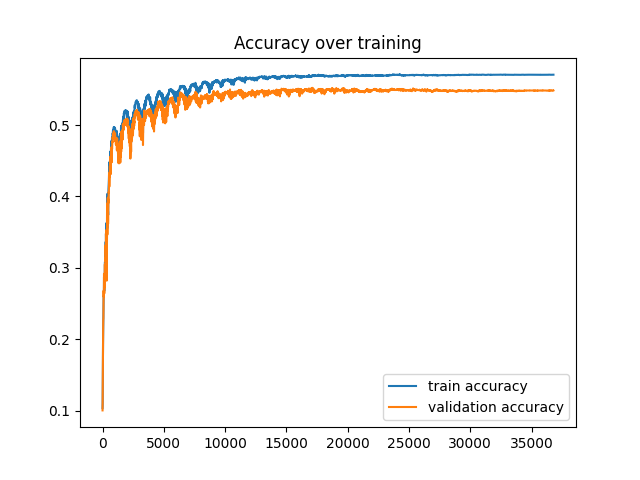
\includegraphics[width=\linewidth]{images/Final_cycle_tracker_acc.png}
		\caption{}
	\end{subfigure}
	\begin{subfigure}{0.3\textwidth}
		\centering
		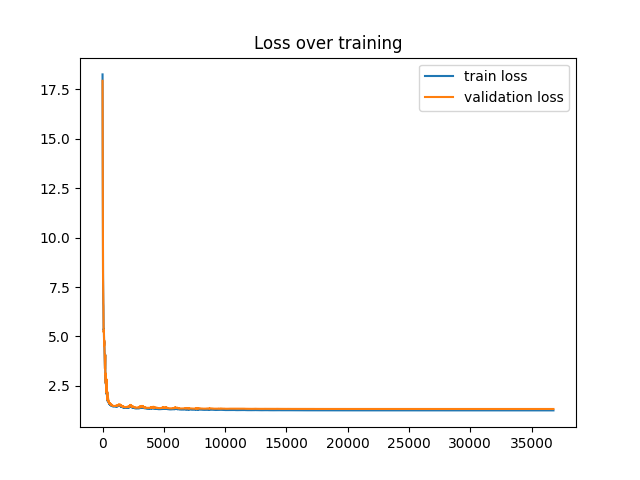
\includegraphics[width=\linewidth]{images/Final_cycle_tracker_loss.png}
		\caption{}
	\end{subfigure}
	\begin{subfigure}{0.3\textwidth}
		\centering
		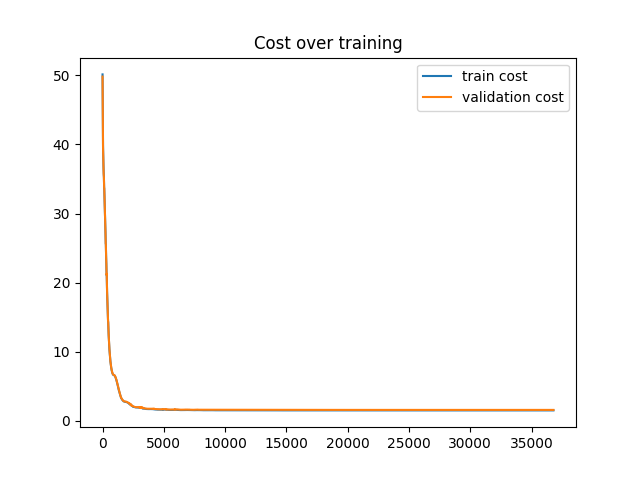
\includegraphics[width=\linewidth]{images/Final_cycle_tracker_cost.png}
		\caption{}
	\end{subfigure}
	\caption{Training of the model with good hyper-parameters for 80 epochs}
	\label{fig:last}
\end{figure}


%%%%%%%% EXTRA TIPS %%%%%%%%
%% If you want to include an figure
%%\begin{figure}[H]
%%\includegraphics[]{Pendulum.jpg}
%%\caption{Sketch of the pendulum}
%%\label{fig:pendulum}
%%\end{figure}

%% for multiple figures in one fig
%\begin{figure}[h]
%	\centering
%	\begin{subfigure}{\textwidth}
%		\centering
%		\includegraphics[width=\linewidth]{images/sthfivo.png}
%		\caption{}
%	\end{subfigure}
%	\begin{subfigure}{\textwidth}
%		\centering
%		\includegraphics[width=\linewidth]{images/sth.png}
%		\caption{}
%	\end{subfigure}
%	\begin{subfigure}{\textwidth}
%		\centering
%		\includegraphics[width=\linewidth]{images/sth.png}
%		\caption{}
%	\end{subfigure}
%	\caption{caption}
%	\label{fig:label}
%\end{figure}


%% You can then reference with \ref{fig:pendulum}


%%\newpage


\end{document}